\documentclass[12pt,fleqn]{article}
\setlength{\parindent}{0pt}
\usepackage{graphicx}
\usepackage{listings}
\usepackage[latin5]{inputenc}
\setlength{\parskip}{8pt}
\setlength{\parsep}{0pt}
\setlength{\headsep}{0pt}
\setlength{\topskip}{0pt}
\setlength{\topmargin}{0pt}
\setlength{\topsep}{0pt}
\setlength{\partopsep}{0pt}
\setlength{\mathindent}{0cm}

\begin{document}
MIT OCW ODE - Ders 12

Bu derste homojen olmayan (inhomogeneous) denklemlere ciddi bir giris
yapacagiz.

\[ y'' + p(x)y' + q(x)y = f(x) \]

Simdiye kadar esitligin sag tarafi s�f�r olmustu, artik orada bir fonksiyon
var. Not: Cogu uygulamada $x$ yerine $t$ sembolu vardir, zaman (time) icin.

$f(x)$ icin pek cok isim kullanilir. Giris sinyali (input signal), surucu
terimi (driving term), guc terimi (forcing term), vs. Bunlardan hangisinin
kullanildigi hangi derste oldugunuza gore degisebilir, farkli muhendislik,
bilim dallari farkli terimleri kullanabilirler, ama tum bu terimler ayni
seyi kastediyorlar. 

Cozum $y(x)$ ise cevap (response) olarak nitelenir, ��kt� (output) kelimesi
de kullanilir. 

Simdiye kadar homojen kosulu incelememizin sebebi ustteki ODE'nin homojen
denklemin cozumu bilinmeden cozulemeyecegi.. Yani $y'' + p(x)y' + q(x)y =
0$ 
denklemi cozum icin onemli. S�f�ra esit olan denkleme de farkli isimler
veriliyor: Alakali homojen ODE, indirgenmis (reduced) denklem gibi.

Yani homojen denklemin cozumu $y = c_1y_1 + c_2y_2$ homojen olmayan denklem
icin gerekli, o sebeple ayri bir sekilde bir sembolu de var. Bazen $y_c$,
bazen $y_h$. Hic alt sembol (subscript) koymayanlar da var, bunlar isi
oldukca karistiriyorlar tabii. $y_c$'ye verilen isim nedir? Bir ismi yok,
cogu kitap ona ``akalali homojen denklemin cozumu'' gibi uzun bir etiket
veriyor. Bu dersin kitabi ona ``tamamlayici cozum (complimentary
solution)'' ismi vermis. 

Klasik Ornekler

\[ mx'' + bx' + kx = f(t) \]

Bu daha onceden hatirlayacagimiz yay / kutle / engelleyici sistemi. Fakat
bu sistemde daha once sag taraf s�f�rdi. Simdi s�f�r yerine olan $f(t)$
fiziksel sistemde neyi temsil ediyor? 

Resmi hatirlayalim

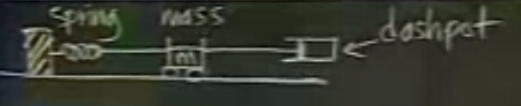
\includegraphics[height=2cm]{12_1.png}

Ortada duran kutle ileri geri gidebiliyordu, eger denklemde $f(t)$ varsa,
biri o kutle uzerinde ek olarak direk bir guc uygulami olur, mesela
kutlenin bir metal oldugunu farzedelim, ve uzaktan birinin bir miknatis
tutarak yay, engelleyici ``haricinde'' degisik bir yonden de bir guc
uyguladigini hayal edelim. 

$f(t)=0$ oldugu zaman (yani denklemde olmadigi zaman), sistem
pasiftir. Disaridan hicbir guc uygulanmamaktadir. 

\end{document}
